\printbibliography
\newpage

\appendix
\noindent
%\twocolumn
\section{Appendix}
\subsection*{Segmentation Models}

\renewcommand{\thefigure}{A\arabic{figure}}
\setcounter{figure}{0}

\begin{figure}[h]
    \begin{tabular}{cc}
    	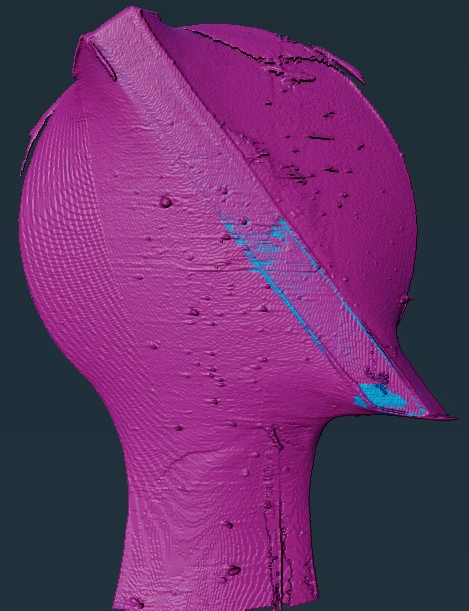
\includegraphics[height=7cm ]{images/avizo_flats/tlys9.jpg} & 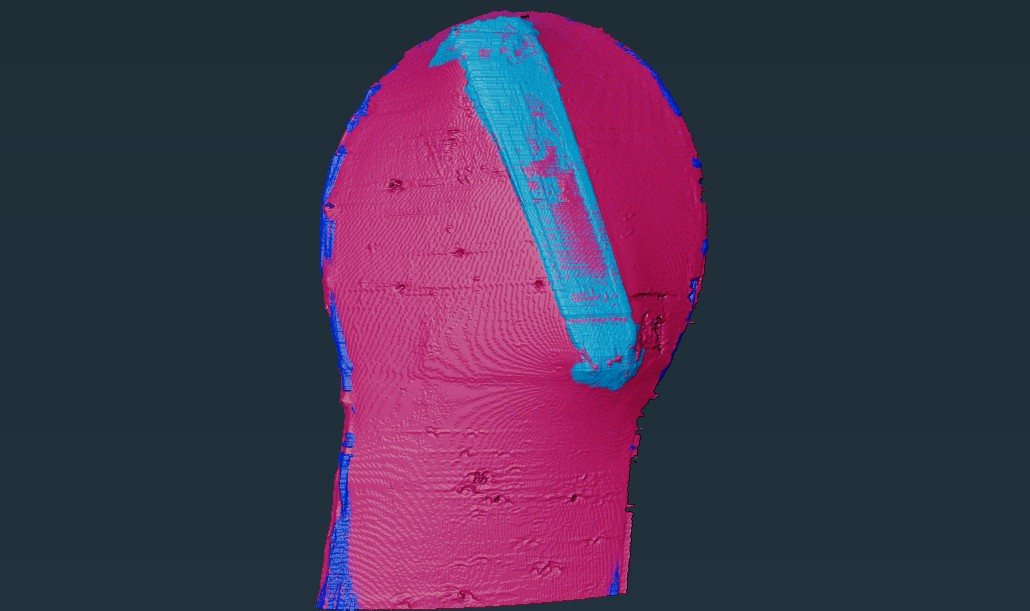
\includegraphics[height=7cm]{images/avizo_flats/tlys2.jpg}
    \end{tabular}
	\caption{Volume rendering in Avizo showing materials of crystal (light blue), liquor (pink), loop (dark blue): Thermolysin 1 (left) and Thermolysin 2 (right)}
 \label{tlys2}
\end{figure}
%\begin{figure}
	%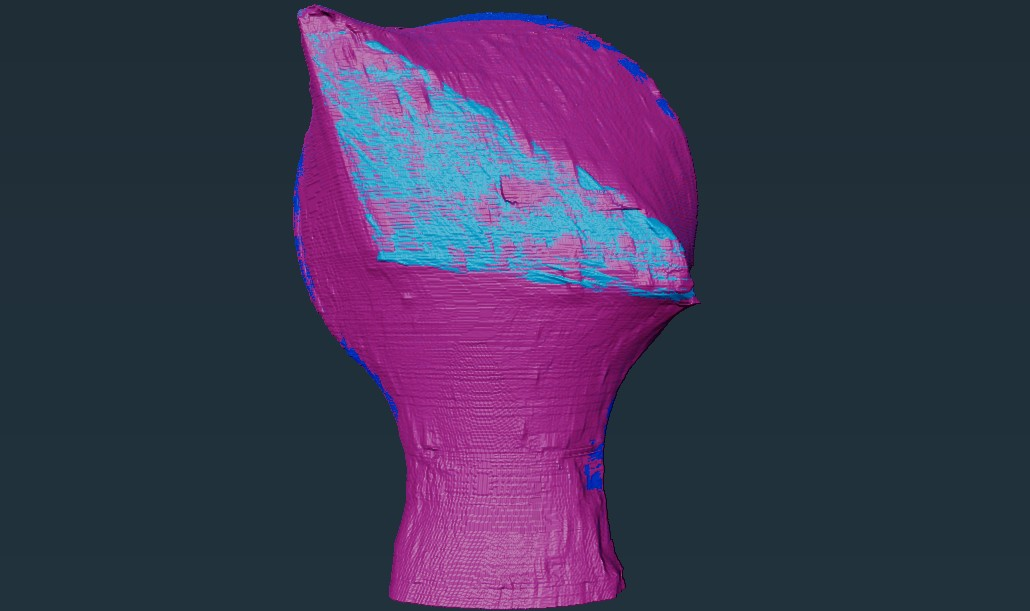
\includegraphics[width=0.5\textwidth]{images/avizo_flats/cas3_1118.jpg}
	%\caption{Volume rendering in Avizo:}
%\label{cas3}
%\end{figure}


\begin{figure}[h]
    \begin{tabular}{cc}
	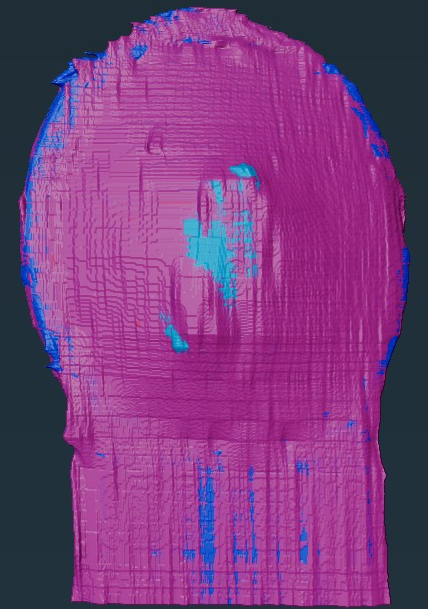
\includegraphics[height=7cm]{images/avizo_flats/ins_con.jpg} & 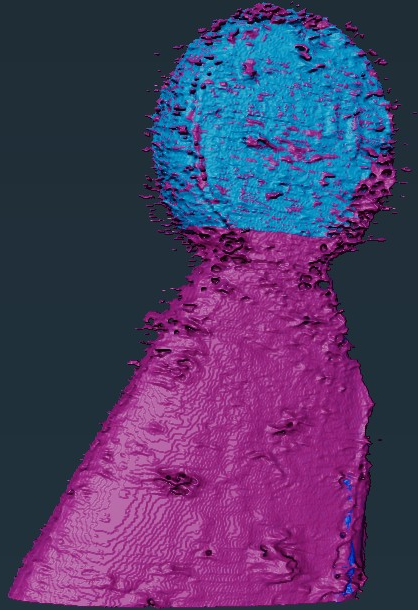
\includegraphics[height=7cm]{images/avizo_flats/ins_ls.jpg}
    \end{tabular}
	\caption{Volume rendering in Avizo showing materials of crystal (light blue), liquor (pink), loop (dark blue): Insulin control crystal (left) and laser-shaped crystal (right)}
 \label{avizo_insulin}
\end{figure}


\begin{figure}
    \begin{tabular}{cc}
	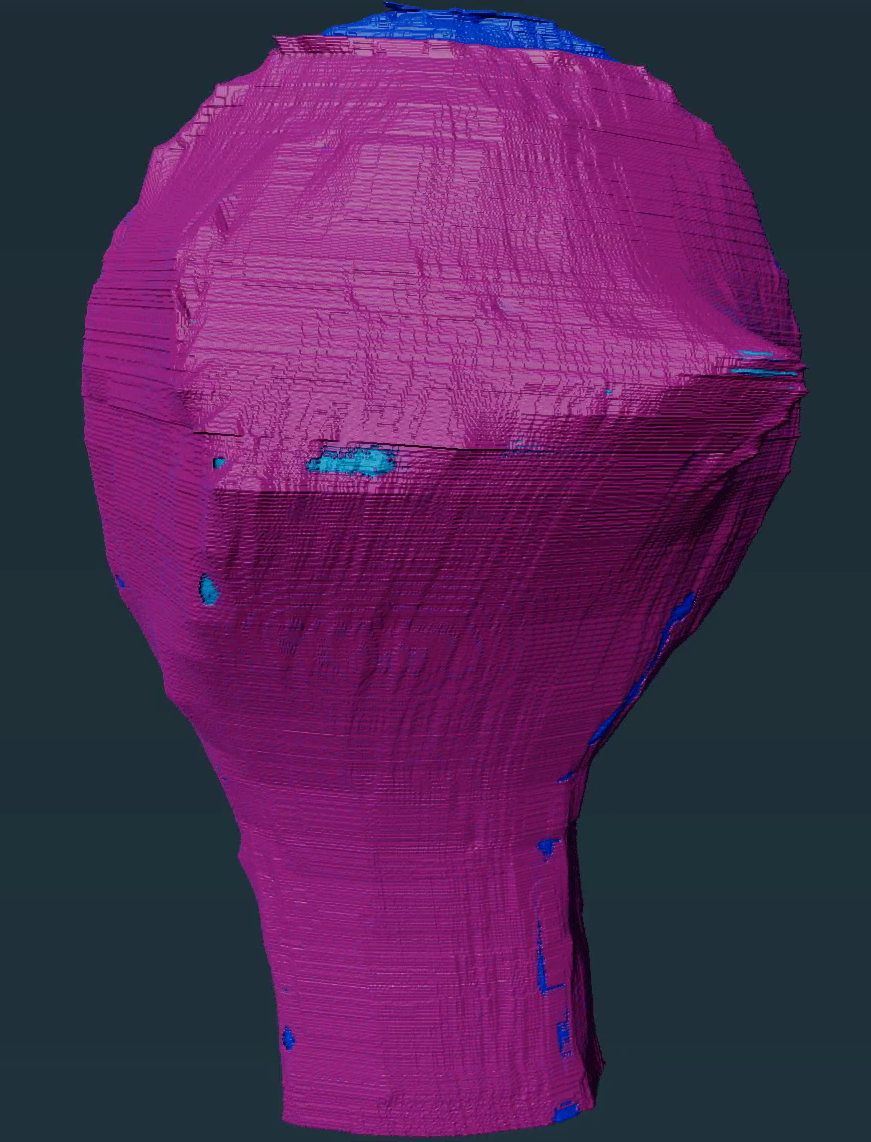
\includegraphics[height=7cm]{images/avizo_flats/prot_con.png} & 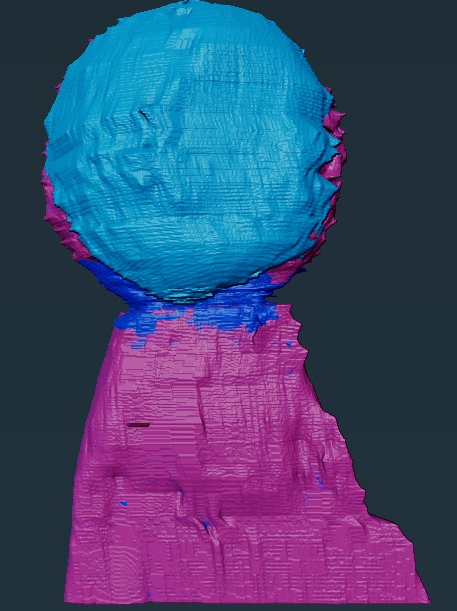
\includegraphics[height=7cm]{images/avizo_flats/prot_ls.jpg}
    \end{tabular}
    \caption{Volume rendering in Avizo showing materials of crystal (light blue), liquor (pink), loop (dark blue): Proteinase-K control crystal (left) and laser-shaped crystal (right)}
    \label{avizo_proteinasek}
\end{figure}


\onecolumn


\newpage

\setcounter{table}{0}
\renewcommand{\thetable}{A\arabic{table}}
\subsection*{Tables}

% Please add the following required packages to your document preamble:
% \usepackage{booktabs}
% \usepackage{multirow}
% \usepackage{graphicx}
% \usepackage[table,xcdraw]{xcolor}
% Beamer presentation requires \usepackage{colortbl} instead of \usepackage[table,xcdraw]{xcolor}
\begin{table}[h]
\resizebox{\textwidth}{!}{%
\begin{tabular}{@{}lllll@{}}
\toprule
Crystal                          & Energy & N.o. datasets & \begin{tabular}[c]{@{}l@{}}Exposure time\\ (s per 0.2 deg)\end{tabular} & Notes                          \\ \midrule
                                 & 3.0    & 4             & 0.35                          &                                \\
                                 & 3.5    & 5             & 0.25                          &                                \\
\multirow{-3}{*}{Thermolysin 1}  & 3.8    & 5             & 0.22                          &                                \\
                                 & 3.0    & 4             & 0.25                          &                                \\
\multirow{-2}{*}{Thermolysin 2}  & 3.5    & 5             & 0.3                           &                                \\
                                 & 3.0    & 1             & 0.3                           &                                \\
\multirow{-2}{*}{Insulin 1}      & 3.5    & 1             & 0.25                          & \multirow{-2}{*}{laser-shaped} \\
                                 & 3.0    & 1             & 0.3                           &                                \\
\multirow{-2}{*}{Insulin 2}      & 3.5    & 1             & 0.25                          & \multirow{-2}{*}{control}      \\
                                 & 3.0    & 1             & 0.3                           &                                \\
\multirow{-2}{*}{Proteinase-K 1} & 3.5    & 1             & 0.25                          & \multirow{-2}{*}{laser-shaped} \\
                                 & 3.0    & 1             & 0.3                           &                                \\
\multirow{-2}{*}{Proteinase-K 2} & 3.5    & 1             & 0.25                          & \multirow{-2}{*}{control}      \\
                                 & 2.4    & 2             & 0.35                          &                                \\
                                 & 3.0    & 2             & 0.3                           &                                \\
\multirow{-3}{*}{Lysozyme}       & 3.5    & 3             & 0.2                           &                                \\
                                 & 3.0    & 1             & 0.35                          &                                \\
                                 & 3.5    & 1             & 0.2                           &                                \\
                                 & 4.0    & 1             & 0.28                          &                                \\
\multirow{-4}{*}{Thaumatin}      & 4.5    & 1             & 0.18                          &       \\
\bottomrule
\end{tabular}%
}

\caption{Tomography Data Collection Parameters; collected using the goniometer at $\kappa$, $\phi$ = 0$\degree$, 0$\degree$ at the I23 endstation, Diamond Light Source, UK.}
\label{tomo_table}
\end{table}


% Please add the following required packages to your document preamble:
% \usepackage{booktabs}
% \usepackage{multirow}
% \usepackage{graphicx}
\begin{table}[]
\resizebox{\textwidth}{!}{%
\begin{tabular}{@{}lllllll@{}}
\toprule
Crystal                    & Energy               & Processing symmetry group & N.o. datasets      & Transmission       & $\kappa$ & $\phi$  \\ \midrule
\multirow{23}{*}{Thermolysin 1} & \multirow{7}{*}{3.0} & \multirow{4}{*}{P6122}     & \multirow{4}{*}{4} & \multirow{4}{*}{5}  & -25 & -100 \\
                           &                      &                           &                    &                    & -40   & 70   \\
                           &                      &                           &                    &                    & -35   & -70  \\
                           &                      &                           &                    &                    & 0     & 0    \\
                           &                      & \multirow{3}{*}{P1}       & \multirow{3}{*}{3} & \multirow{3}{*}{5} & -70   & 0    \\
                           &                      &                           &                    &                    & -70   & 120  \\
                           &                      &                           &                    &                    & -70   & -120 \\ \cmidrule(l){2-7} 
                           & \multirow{8}{*}{3.5} & \multirow{5}{*}{P6122}    & \multirow{5}{*}{5} & \multirow{5}{*}{1} & 0     & 0    \\
                           &                      &                           &                    &                    & -15   & 100  \\
                           &                      &                           &                    &                    & -25   & -100 \\
                           &                      &                           &                    &                    & -40   & 70   \\
                           &                      &                           &                    &                    & -35   & -70  \\
                           &                      & \multirow{3}{*}{P1}       & \multirow{3}{*}{3} & \multirow{3}{*}{1} & -70   & -120 \\
                           &                      &                           &                    &                    & -70   & 0    \\
                           &                      &                           &                    &                    & -70   & 120  \\ \cmidrule(l){2-7} 
                           & \multirow{8}{*}{3.8} & \multirow{5}{*}{P6122}    & \multirow{5}{*}{5} & \multirow{5}{*}{1} & 0     & 0    \\
                           &                      &                           &                    &                    & -15   & 100  \\
                           &                      &                           &                    &                    & -25   & -100 \\
                           &                      &                           &                    &                    & -40   & 70   \\
                           &                      &                           &                    &                    & -35   & -70  \\ \cmidrule(l){3-7} 
                           &                      & \multirow{3}{*}{P1}       & \multirow{3}{*}{3} & \multirow{3}{*}{1} & -70   & -120 \\
                           &                      &                           &                    &                    & -70   & 0    \\
                           &                      &                           &                    &                    & -70   & 120  \\ \midrule
\multirow{9}{*}{Thermolysin 2}  & \multirow{4}{*}{3.0} & \multirow{4}{*}{P6122, P1} & \multirow{4}{*}{4} & \multirow{4}{*}{20} & 0   & 0    \\
                           &                      &                           &                    &                    & -70   & -100 \\
                           &                      &                           &                    &                    & -70   & 0    \\
                           &                      &                           &                    &                    & -70   & 100  \\ \cmidrule(l){2-7} 
                                & \multirow{5}{*}{3.5} & \multirow{5}{*}{P6122, P1} & \multirow{5}{*}{5} & \multirow{5}{*}{15} & 0   & 0    \\
                           &                      &                           &                    &                    & -70   & -100 \\
                           &                      &                           &                    &                    & -70   & 0    \\
                           &                      &                           &                    &                    & -70   & 100  \\
                           &                      &                           &                    &                    & 0     & 0    \\ \midrule
Insulin 1                  & 3.0                  & I213                      & 1                  & 20                 & 0     & 0    \\ \midrule
Insulin 2                  & 3.0                  & I213                      & 1                  & 15                 & 0     & 0    \\ \midrule
Proteinase-K 1             & 3.0                  & P43212                    & 1                  & 20                 & 0     & 0    \\ \midrule
Proteinase-K 2             & 3.0                  & P43212                    & 1                  & 20                 & 0     & 0    \\ \midrule
\multirow{4}{*}{Thaumatin} & 3.0                  & \multirow{4}{*}{P41212}   & 1                  &                    & 0     & 0    \\
                           & 3.5                  &                           & 1                  &                    & 0     & 0    \\
                           & 4.0                  &                           & 1                  &                    & 0     & 0    \\
                           & 4.5                  &                           & 1                  &                    & 0     & 0    \\ \bottomrule
\end{tabular}%
}
\caption{Diffraction Data Parameters; collected at beamline I23, Diamond Light Source, UK.}
\label{diffration_table}
\end{table}

%\caption{Diffraction Data Collection Parameters}












% Please add the following required packages to your document preamble:
% \usepackage{booktabs}
% \usepackage{multirow}
% \usepackage{graphicx}
% Please add the following required packages to your document preamble:
% \usepackage{booktabs}
% \usepackage{multirow}
% \usepackage{graphicx}
\begin{table}[H]
\resizebox{\textwidth}{!}{%
\begin{tabular}{@{}llllll@{}}
\toprule
\multirow{3}{*}{Element, Energy} &
  \multirow{3}{*}{Theoretical $f'$} &
  \multirow{3}{*}{Theoretical $f"$} &
  \multicolumn{3}{c}{Experimental $f"$} \\
                             &                            &                           & \multicolumn{1}{c}{AC} & \multicolumn{1}{c}{SH} & \multicolumn{1}{c}{ACSH} \\ \cmidrule(l){4-6} 
                             &                            &                           & \multicolumn{3}{c}{\% Difference}                                          \\ \midrule
\multirow{2}{*}{S, 3 \unit{keV}}    & \multirow{2}{*}{-0.75226}  & \multirow{2}{*}{3.059391} & 2.49912                & 2.45008                & 3.03552                  \\
                             &                            &                           & -18.3132               & -19.9161               & -0.78025                 \\ \midrule
\multirow{2}{*}{Zn, 3.0 \unit{keV}} & \multirow{2}{*}{3.56E-02}  & \multirow{2}{*}{3.764636} & 2.83766                & 2.36456                & 2.68316                  \\
                             &                            &                           & -24.6233               & -37.1902               & -28.7272                 \\ \midrule
\multirow{2}{*}{S, 3.5 \unit{keV}}  & \multirow{2}{*}{-8.16E-02} & \multirow{2}{*}{2.390438} & 2.21949                & 2.24339                & 2.42956                  \\
                             &                            &                           & -7.15133               & -6.15151               & 1.636604                 \\ \midrule
\multirow{2}{*}{Zn, 3.5 \unit{keV}}  & \multirow{2}{*}{-6.15E-02} & \multirow{2}{*}{2.912471} & 2.36736                & 2.1546                 & 2.62166                  \\
                             &                            &                           & -18.7164               & -26.0216               & -9.98503                 \\ \bottomrule
\end{tabular}%
}

\caption{Phenix Refinement on three sets of Thermolysin 2 reflection data (corrected by \ac{ac}, \ac{sh}, \ac{acsh}), for sulphur and zinc at 3.0, 3.5 \unit{keV}. Experimentally calculated $f"$ coefficients for a given element and energy are refined based on the theoretical $f'$ and are displayed in the upper bound of the correction methods column. Percentage differences between the theoretical $f"$ and experimental $f"$ across the three methods are displayed in the lower bound.}
\label{phenix_table}
\end{table}


\newpage
\subsection*{Charts \& Plots}

\begin{figure}[h]
    \centering
    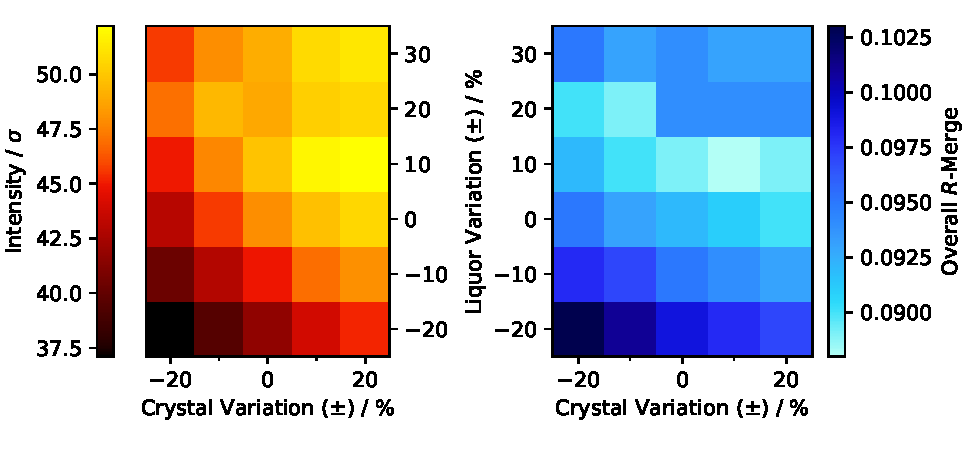
\includegraphics[width = 0.8\textwidth]{plots/exp0/cld_merged_stats.pdf} 
    \caption{Merging statistics showing the effects of varying the experimental Cld crystal and liquor absorption coefficients in Lu \textit{et al.} \cite{Lu2024} calculated by AnACor. Ratio of signal intensities to their uncertainties shown on the left; Global $R_{merge}$ factor shown on the right. (Light shades indicate the best merging statistics, and \textit{vice versa}.)}
    \label{fig:cld_stats}
\end{figure}

\begin{figure}[h]
    \centering
    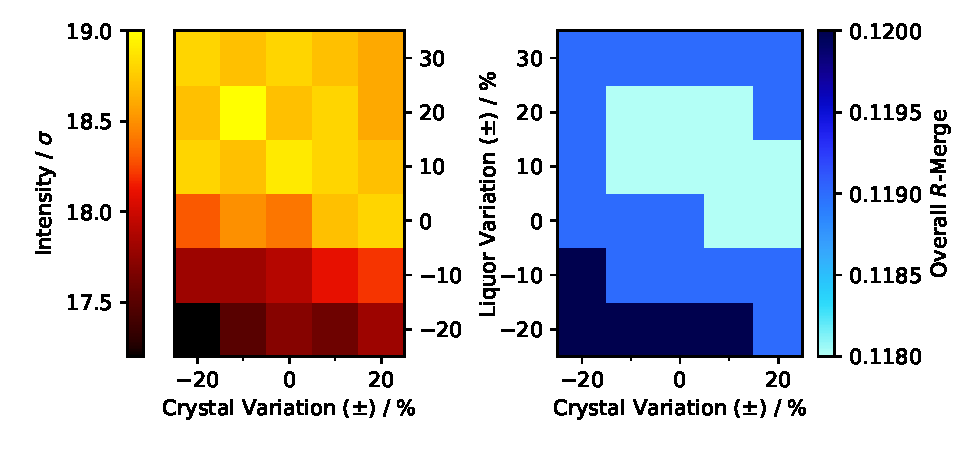
\includegraphics[width = 0.8\textwidth]{plots/exp0/ompk_merged_stats.pdf}
    \caption{Merging statistics showing the effects of varying the experimental Ompk crystal and liquor absorption coefficients in Lu \textit{et al.} \cite{Lu2024} calculated by AnACor. Ratio of signal intensities to their uncertainties shown on the left; Global $R_{merge}$ factor shown on the right. (Light shades indicate the best merging statistics, and \textit{vice versa}.)}
    \label{fig:ompk_stats}
\end{figure}



\begin{figure}[h]
    \centering
    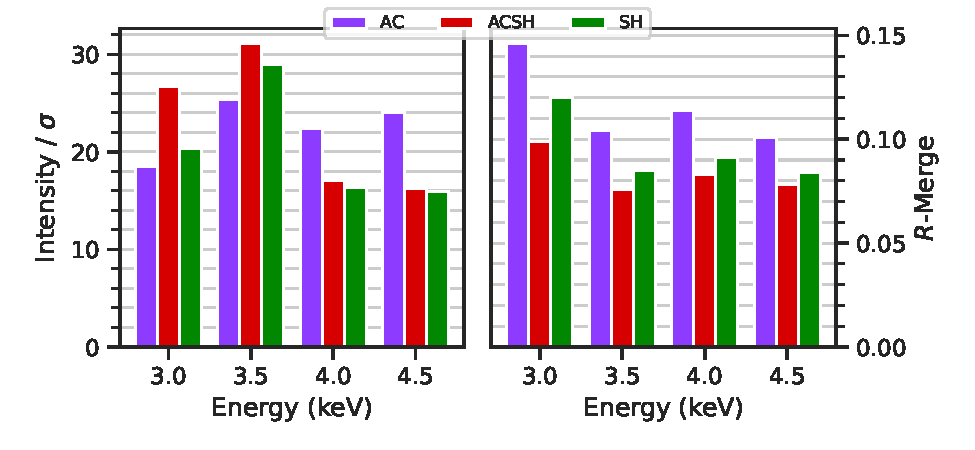
\includegraphics{plots/exp0/thaum_stats_grid.pdf}
    \caption{Merging statistics for thaumatin protein crystal. Ratio of signal intensities to their uncertainties shown on the left; Global $R_{merge}$ factor shown on the right.}
    \label{fig:thaum1_stats}
\end{figure}


\newpage
%\section{Plots}

%TLYS 9 Merging STATS
\begin{figure}
    \centering
    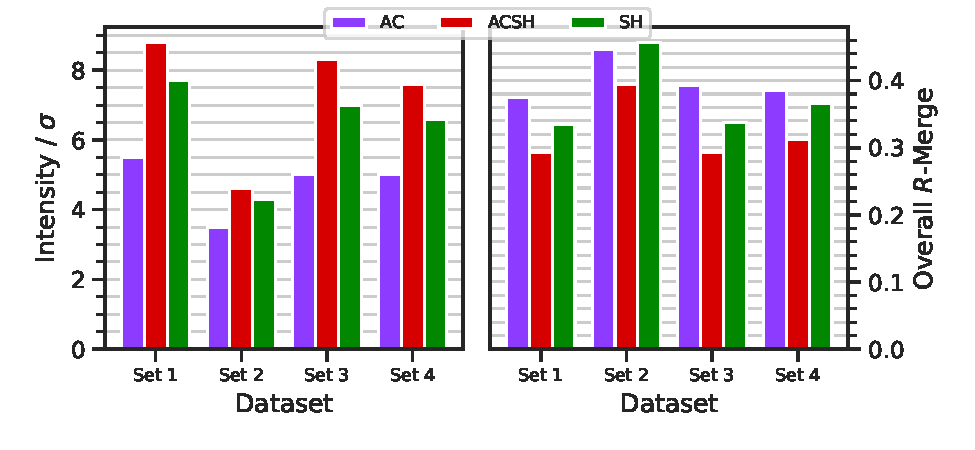
\includegraphics{plots/exp1/tlys_9_P6122/3p0_stats_grid.pdf}
    \caption{Merging statistics for Thermolysin 1 at 3.0 \unit{keV}. Ratio of signal intensities to their uncertainties shown on the left; Global $R_{merge}$ factor shown on the right.}
    \label{fig:tlys_9_3p0}
\end{figure}

\begin{figure}
    \centering
    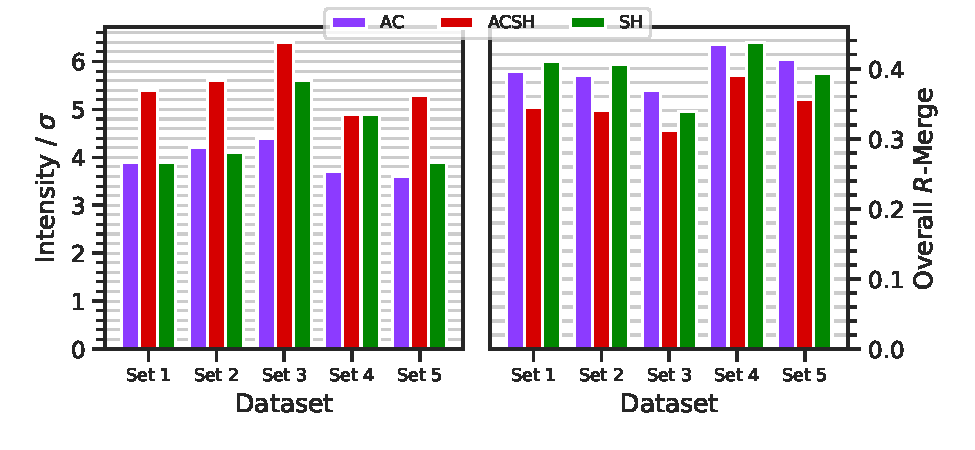
\includegraphics{plots/exp1/tlys_9_P6122/3p5_stats_grid.pdf}
    \caption{Merging statistics for Thermolysin 1 at 3.5 \unit{keV}. Ratio of signal intensities to their uncertainties shown on the left; Global $R_{merge}$ factor shown on the right.}
    \label{fig:tlys_9_3p5}
\end{figure}

\begin{figure}
    \centering
    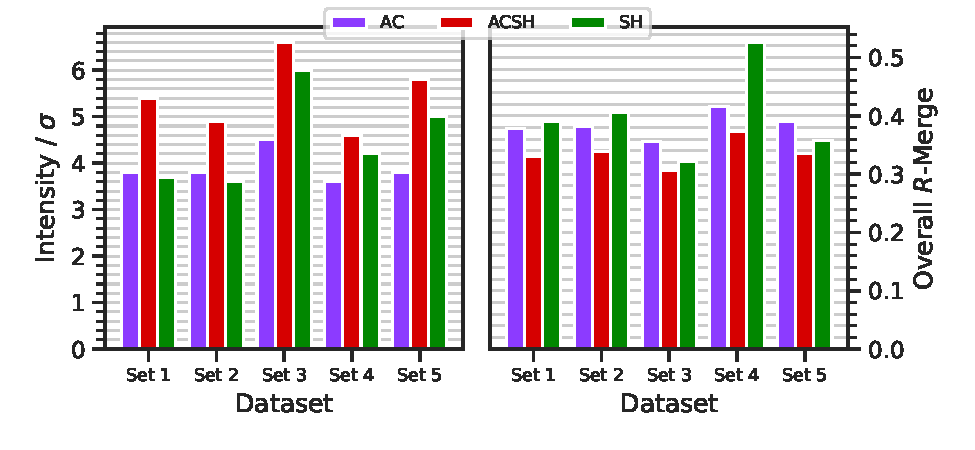
\includegraphics{plots/exp1/tlys_9_P6122/3p8_stats_grid.pdf}
    \caption{Merging statistics for Thermolysin 1 at 3.8 \unit{keV}. Ratio of signal intensities to their uncertainties shown on the left; Global $R_{merge}$ factor shown on the right.}
    \label{fig:tlys_9_3p8}
\end{figure}

% TLYS 2 MERGING STATS

\begin{figure}
    \centering
    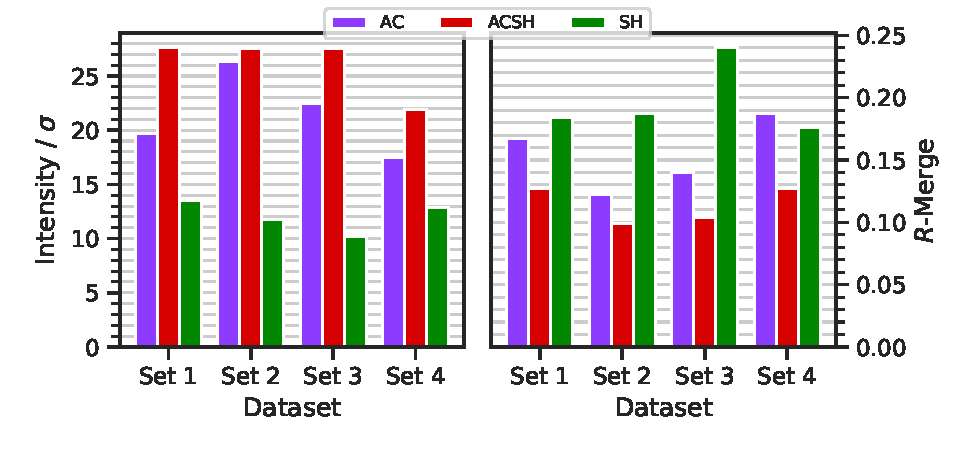
\includegraphics{plots/exp1/tlys_2_P6122/3p0_stats_grid.pdf}
    \caption{Merging statistics for Thermolysin 2 at 3.0 \unit{keV}. Ratio of signal intensities to their uncertainties shown on the left; Global $R_{merge}$ factor shown on the right.}
    \label{fig:tlys_2_3p0}
\end{figure}

\begin{figure}
    \centering
    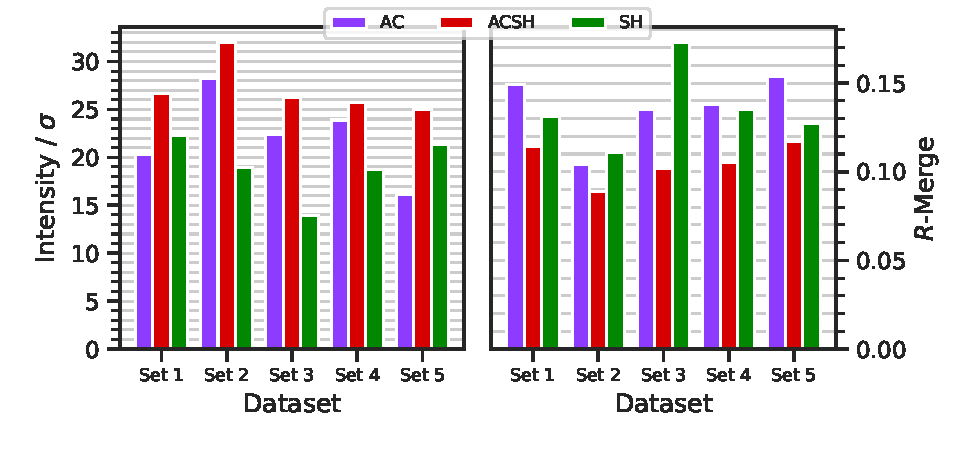
\includegraphics{plots/exp1/tlys_2_P6122/3p5_stats_grid.pdf}
    \caption{Merging statistics for Thermolysin 2 at 3.5 \unit{keV}. Ratio of signal intensities to their uncertainties shown on the left; Global $R_{merge}$ factor shown on the right.}
    \label{fig:tlys_2_3p5}
\end{figure}


% TLYS 9 ANODE PEAKS
\begin{figure}
    \centering
    \begin{tabular}{cc}
        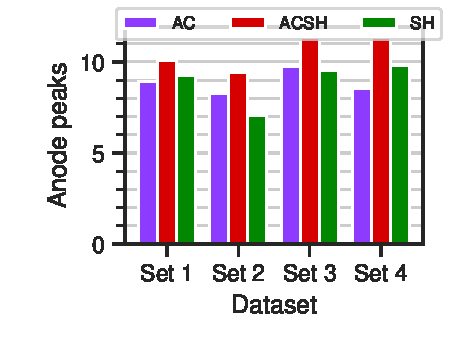
\includegraphics[width = 0.5\textwidth]{plots/exp1/tlys_9_P6122/peaks/3p0_met250.pdf} & 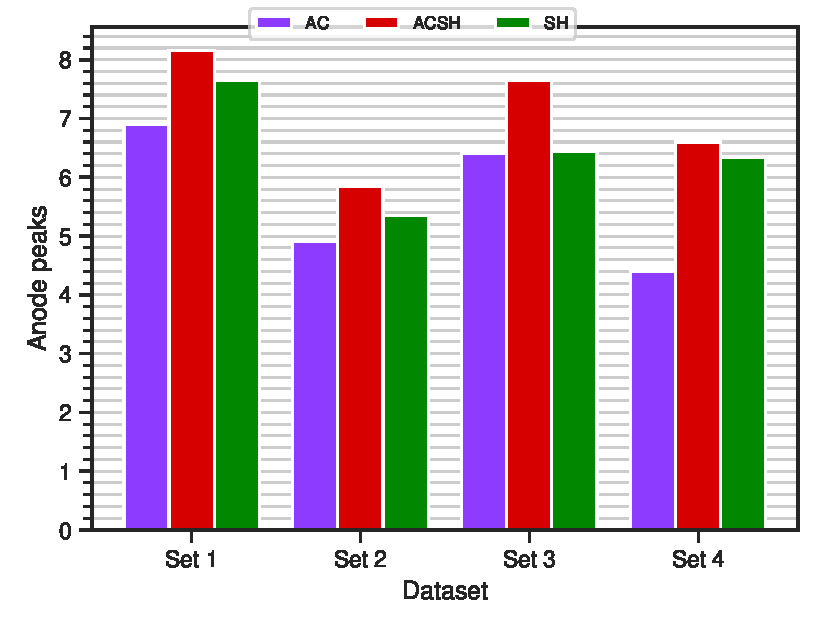
\includegraphics[width = 0.5\textwidth]{plots/exp1/tlys_9_P6122/peaks/3p0_met120.pdf}
    \end{tabular}
    \caption{Thermolysin 1: Anomalous density peaks of methionine groups at 3.0 \unit{keV}. Methionine in polypeptide chain position 205 shown on the left. Methionine in position 120 shown on the right.}
    \label{fig:tlys9_met_peaks_3p0}
\end{figure}

\begin{figure}
    \centering
    \begin{tabular}{cc}
        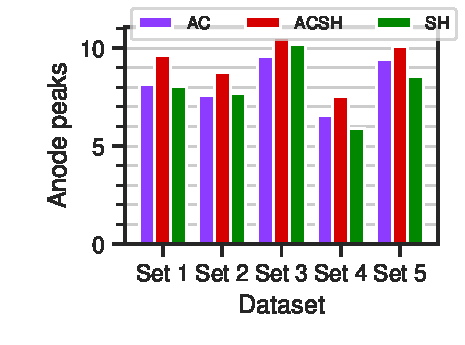
\includegraphics[width = 0.5\textwidth]{plots/exp1/tlys_9_P6122/peaks/3p5_met250.pdf} & 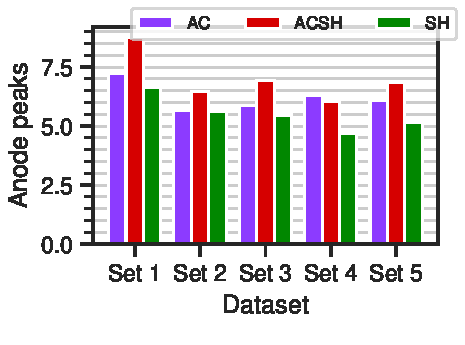
\includegraphics[width = 0.5\textwidth]{plots/exp1/tlys_9_P6122/peaks/3p5_met120.pdf}
    \end{tabular}
    \caption{Thermolysin 1: Anomalous density peaks of methionine groups at 3.5 \unit{keV}. Methionine in polypeptide chain position 205 shown on the left. Methionine in position 120 shown on the right.}
    \label{fig:tlys9_met_peaks_3p5}
\end{figure}

\begin{figure}
    \centering
    \begin{tabular}{cc}
        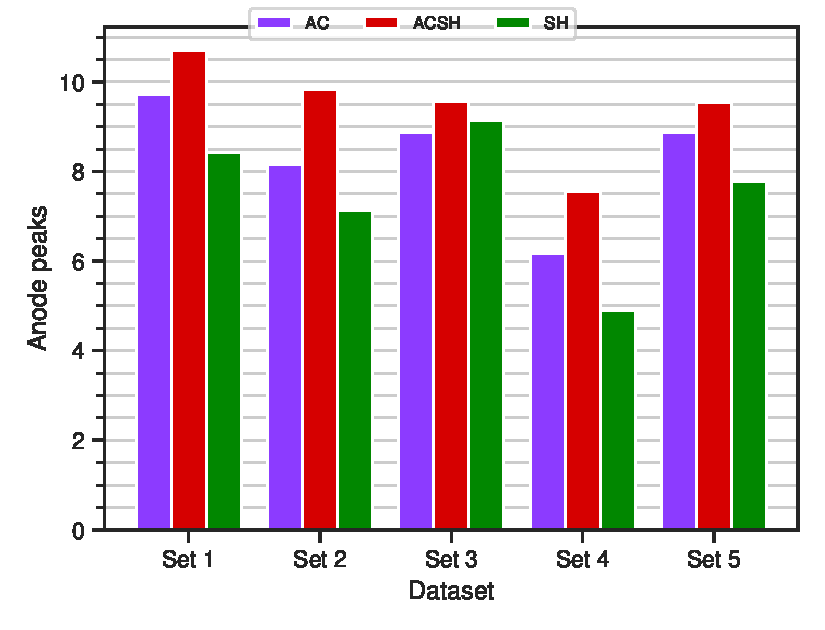
\includegraphics[width = 0.5\textwidth]{plots/exp1/tlys_9_P6122/peaks/3p8_met250.pdf} & 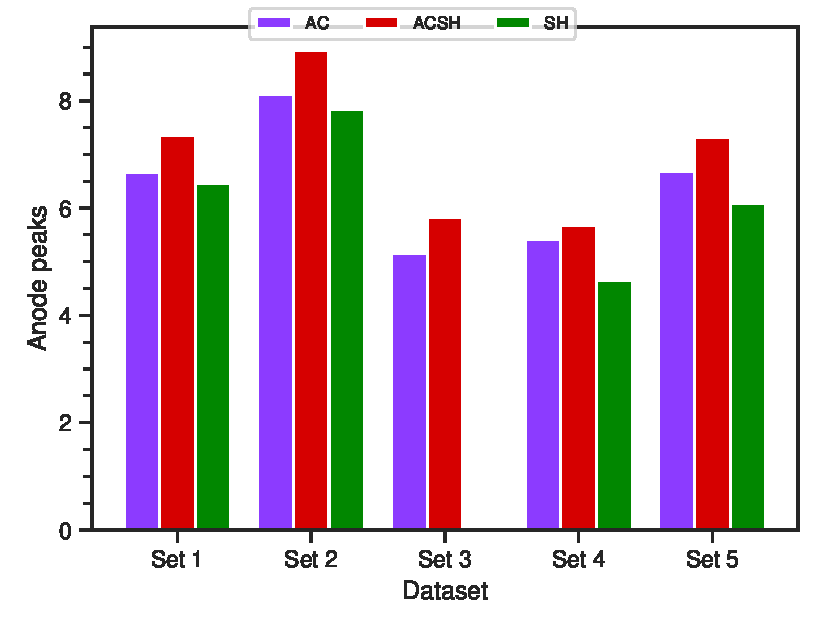
\includegraphics[width = 0.5\textwidth]{plots/exp1/tlys_9_P6122/peaks/3p8_met120.pdf}
    \end{tabular}
    \caption{Thermolysin 1: Anomalous density peaks of methionine groups at 3.8 \unit{keV}. Methionine in polypeptide chain position 205 shown on the left. Methionine in position 120 shown on the right.}
    \label{fig:tlys9_met_peaks_3p8}
\end{figure}

\begin{figure}
    \centering
    \begin{tabular}{cc}
        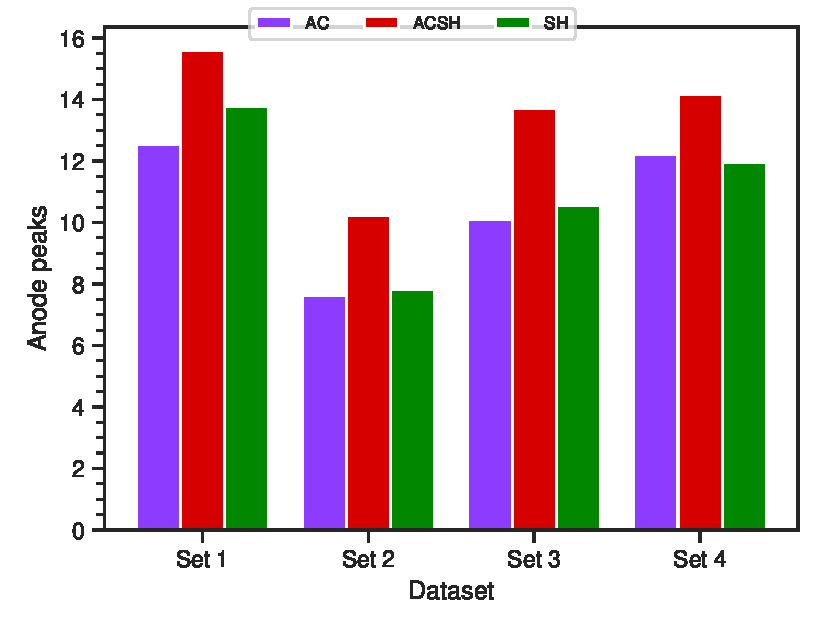
\includegraphics[width = 0.5\textwidth]{plots/exp1/tlys_9_P6122/peaks/3p0_zinc.pdf} & 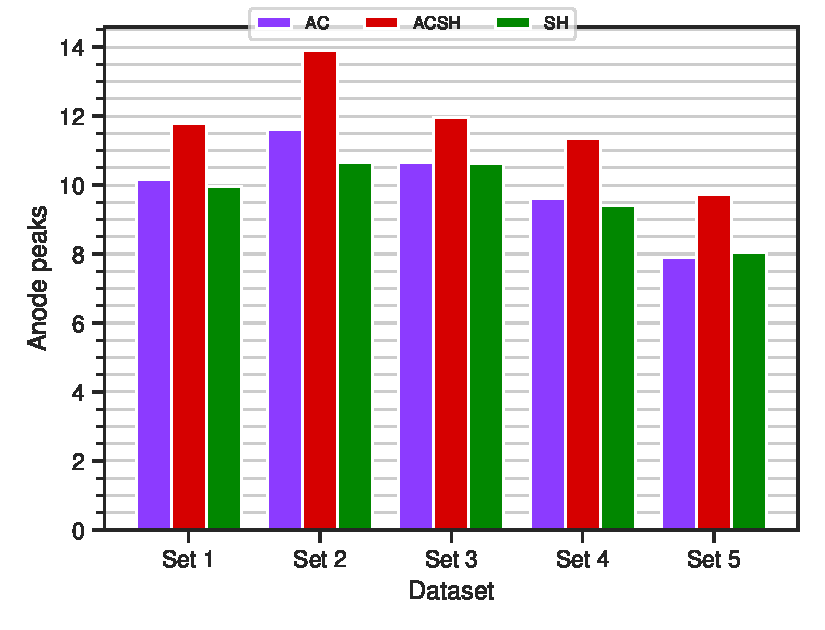
\includegraphics[width = 0.5\textwidth]{plots/exp1/tlys_9_P6122/peaks/3p5_zinc.pdf}
    \end{tabular}
    \caption{Thermolysin 1: Anomalous density peaks of zinc at 3.0 \unit{keV} (left) and 3.5 \unit{keV} (right).}
    \label{fig:tlys9_zn_peaks_3p0_3p5}
\end{figure}

\begin{figure}
    \centering
    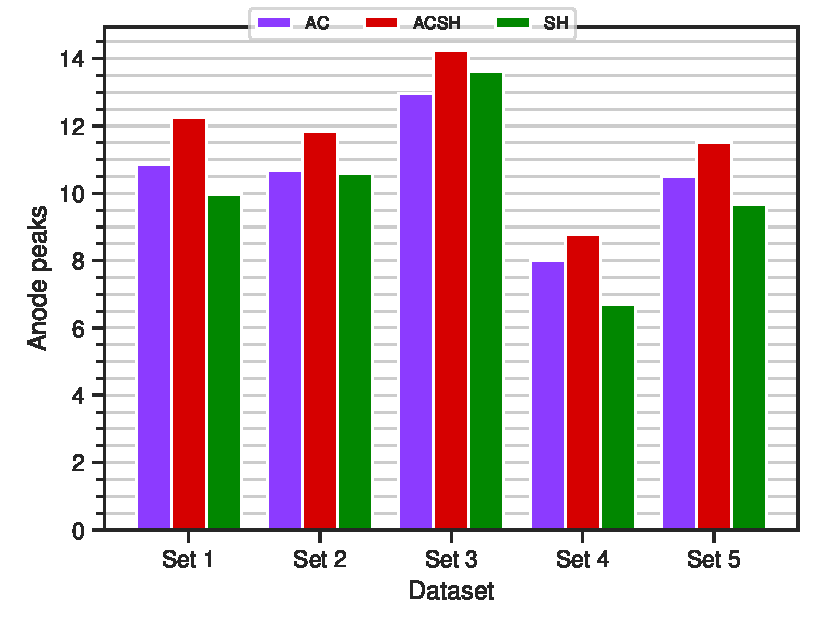
\includegraphics[width = 0.5\textwidth]{plots/exp1/tlys_9_P6122/peaks/3p8_zinc.pdf}
    \caption{Thermolysin 1: Anomalous density peaks of Zinc at 3.8 \unit{keV}.}
    \label{fig:tlys9_zn_peaks_3p8}
\end{figure}


%P1
\begin{figure}[]
    \centering
    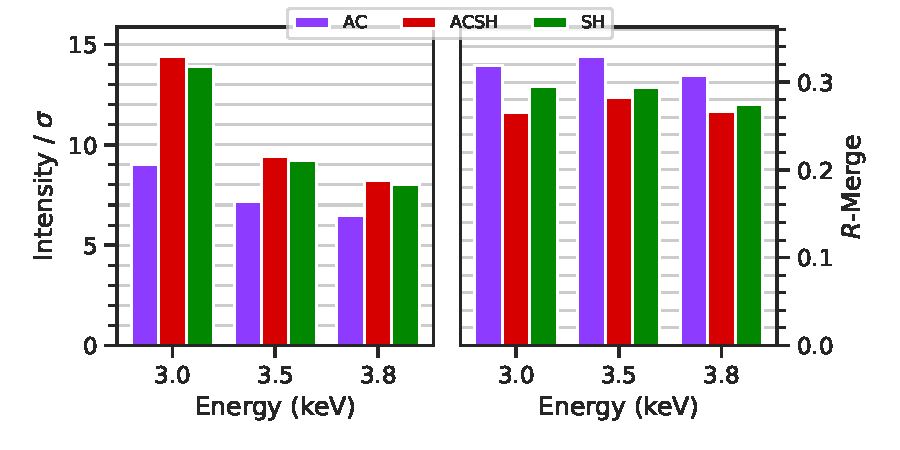
\includegraphics{plots/exp1/tlys_9_P1/merged_stats.pdf}
    \caption{Merging statistics for Thermolysin 1 processed in $P_1$. Ratio of signal intensities to their uncertainties shown on the left; Global $R_{merge}$ factor shown on the right.}
    \label{fig:tlys_9_p1}
\end{figure}

\begin{figure}[]
    \centering
    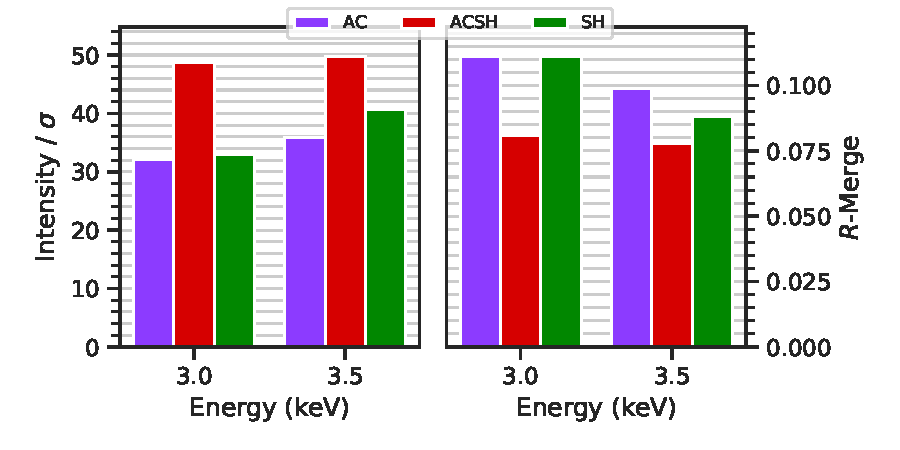
\includegraphics{plots/exp1/tlys_2_P1/stats.pdf}
    \caption{Merging statistics for Thermolysin 2 processed in $P_1$. Ratio of signal intensities to their uncertainties shown on the left; Global $R_{merge}$ factor shown on the right.}
    \label{fig:tlys_2_p1}
\end{figure}




% TLYS 2 ANODE PEAKS
\begin{figure}
    \centering
    \begin{tabular}{cc}
        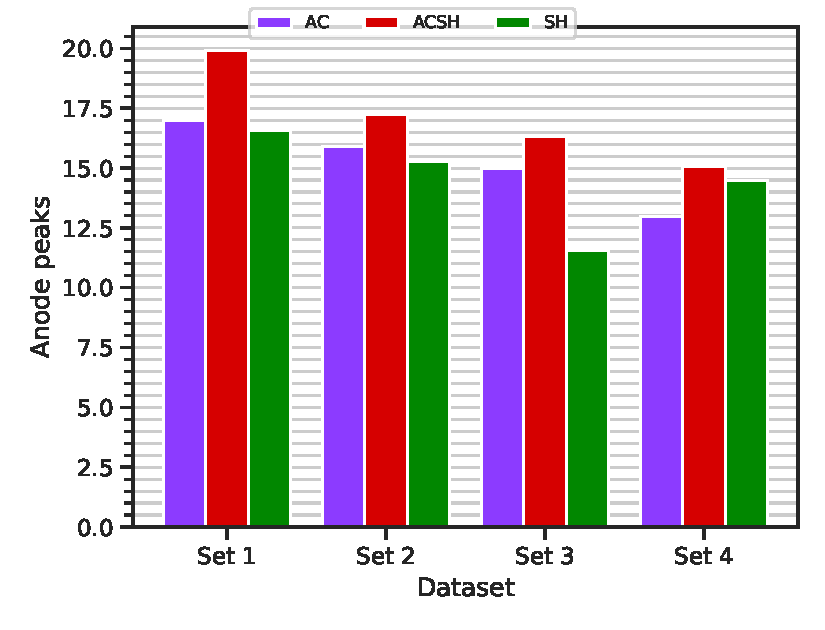
\includegraphics[width = 0.5\textwidth]{plots/exp1/tlys_2_P6122/peaks/3p0_met250.pdf} & 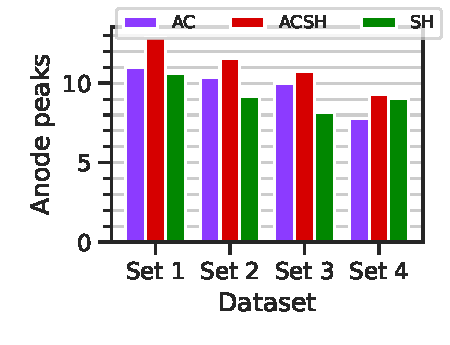
\includegraphics[width = 0.5\textwidth]{plots/exp1/tlys_2_P6122/peaks/3p0_met120.pdf}
    \end{tabular}
    \caption{Thermolysin 2: Anomalous density peaks of methionine groups at 3.0 \unit{keV}. Methionine in polypeptide chain position 205 shown on the left. Methionine in position 120 shown on the right.}
    \label{fig:tlys2_met_peaks_3p0}
\end{figure}

\begin{figure}
    \centering
    \begin{tabular}{cc}
        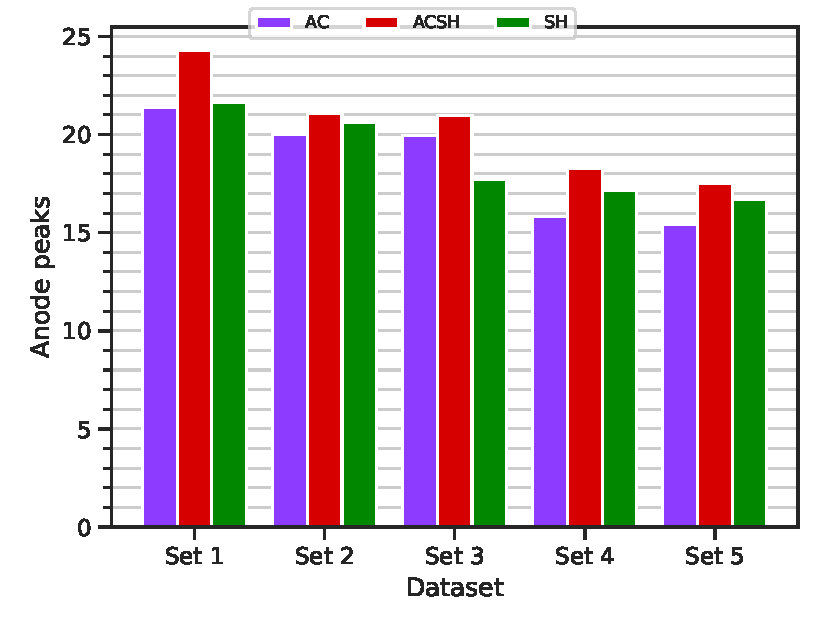
\includegraphics[width = 0.5\textwidth]{plots/exp1/tlys_2_P6122/peaks/3p5_met250.pdf} & 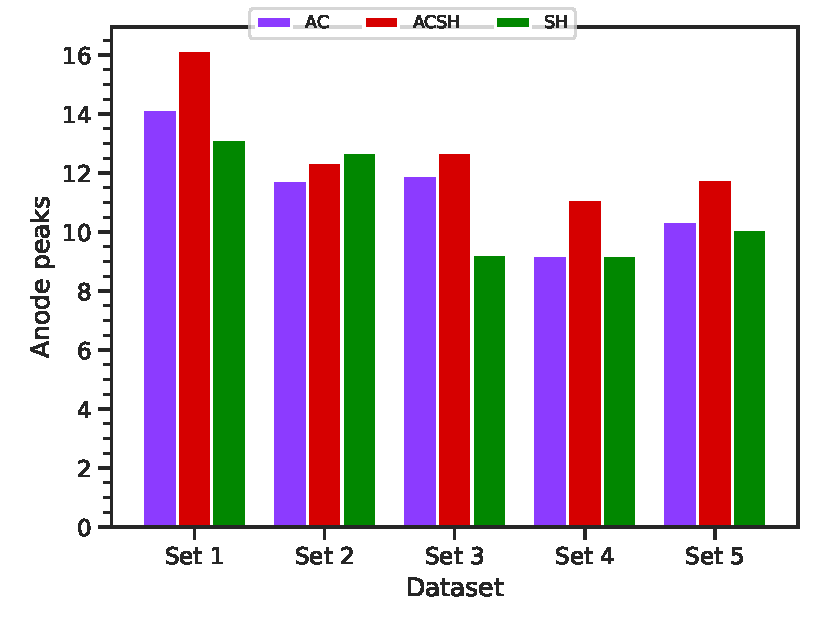
\includegraphics[width = 0.5\textwidth]{plots/exp1/tlys_2_P6122/peaks/3p5_met120.pdf}
    \end{tabular}
    \caption{Thermolysin 2: Anomalous density peaks of methionine groups at 3.5 \unit{keV}. Methionine in polypeptide chain position 205 shown on the left. Methionine in position 120 shown on the right.}
    \label{fig:tlys2_met_peaks_3p5}
\end{figure}

\begin{figure}
    \centering
    \begin{tabular}{cc}
        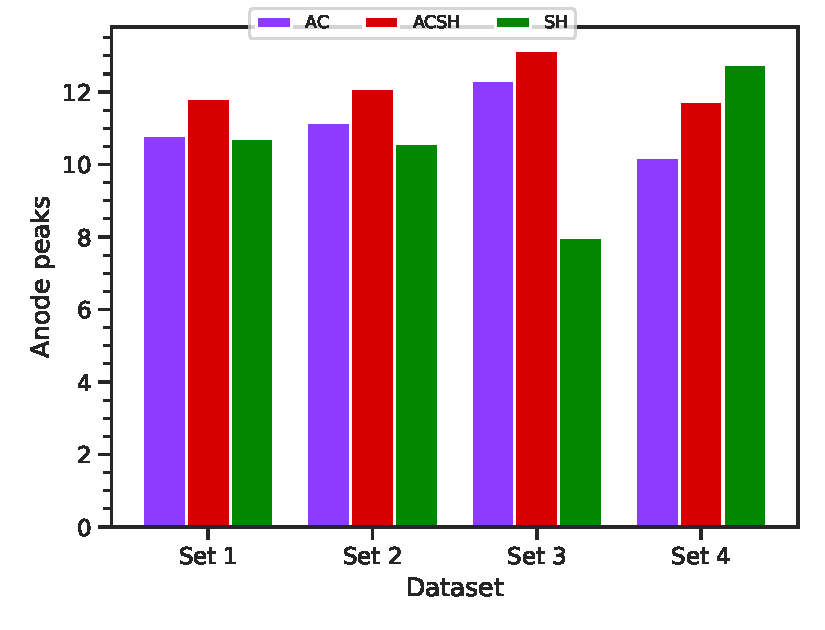
\includegraphics[width = 0.5\textwidth]{plots/exp1/tlys_2_P6122/peaks/3p0_zinc.pdf} & 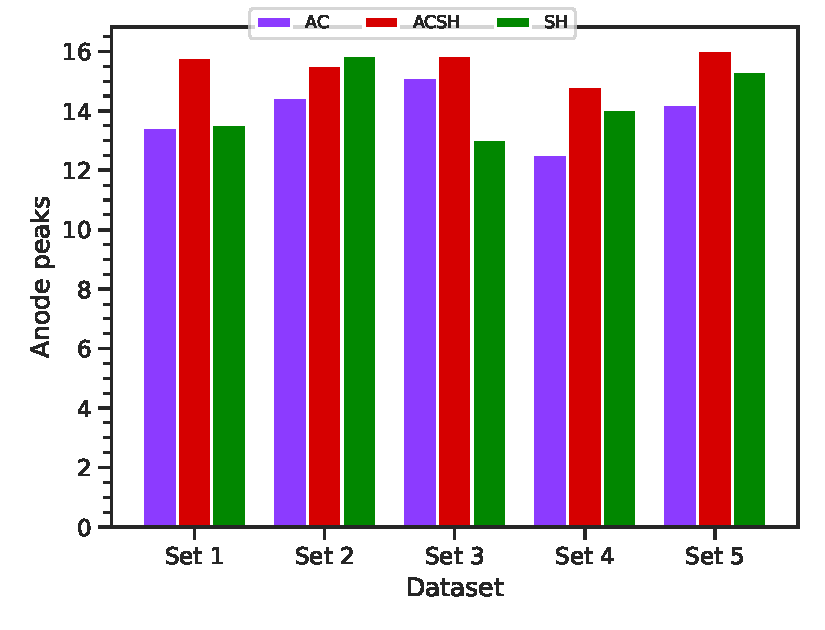
\includegraphics[width = 0.5\textwidth]{plots/exp1/tlys_2_P6122/peaks/3p5_zinc.pdf}
    \end{tabular}
    \caption{Thermolysin 2: Anomalous density peaks of zinc at 3.0 \unit{keV} (left) and 3.5 \unit{keV} (right).}
    \label{fig:tlys2_zn_peaks}
\end{figure}